\documentclass[a4paper, 12pt]{article}
\usepackage[total={17cm,25cm}, top=2.5cm, left=2.5cm, right=2.5cm,  includefoot]{geometry}
\usepackage[utf8]{inputenc}
\usepackage{array}
\usepackage{multirow}
\usepackage{hhline}
\usepackage{gensymb}
\usepackage{graphicx}
\graphicspath{ {} }
\usepackage[czech]{babel}
\usepackage{enumitem}
\usepackage{pdfpages}
\usepackage{amsmath}
\usepackage{verbatim}
\usepackage{listings}
\usepackage{hyperref}
\usepackage{amssymb}


\pagestyle{empty} % vypne číslování stránek




\usepackage[OT2,OT1]{fontenc}
\newcommand\cyr
{
\renewcommand\rmdefault{wncyr}
\renewcommand\sfdefault{wncyss}
\renewcommand\encodingdefault{OT2}
\normalfont
\selectfont
}
\DeclareTextFontCommand{\textcyr}{\cyr}
\def\cprime{\char"7E }
\def\cdprime{\char"7F }
\def\eoborotnoye{\char’013}
\def\Eoborotnoye{\char’003}
\setlength{\parindent}{1em} 
%\setlength{\parskip}{0.5ex}


\begin{document}

\begin{titlepage}
\begin{center}
\Huge
\vspace*{4.5cm}
Algoritmy v digitální kartografii\\
\vspace{0.2cm}

\Large  
Digitální model terénu a jeho analýzy\\
\vspace{0.2cm}

\normalsize  
Zimní semestr 2018/2019\\
%(oprava: 24. 11. 2018)
\vspace{14cm}
\end{center}

\begin{flushright}
\Large
Tereza Kulovaná \\
Markéta Pecenová \\
\end{flushright}

\end{titlepage}


\pagestyle{plain}     % zapne obyčejné číslování
\setcounter{page}{1}  % nastaví čítač stránek znovu od jedné

\tableofcontents
\newpage

\section{Zadání}
Zadání úlohy bylo staženo ze stránek předmětu \href{https://web.natur.cuni.cz/~bayertom/index.php/teaching/algoritmy-v-digitalni-kartografii}{155ADKG}.

\begin{figure}[h!]
	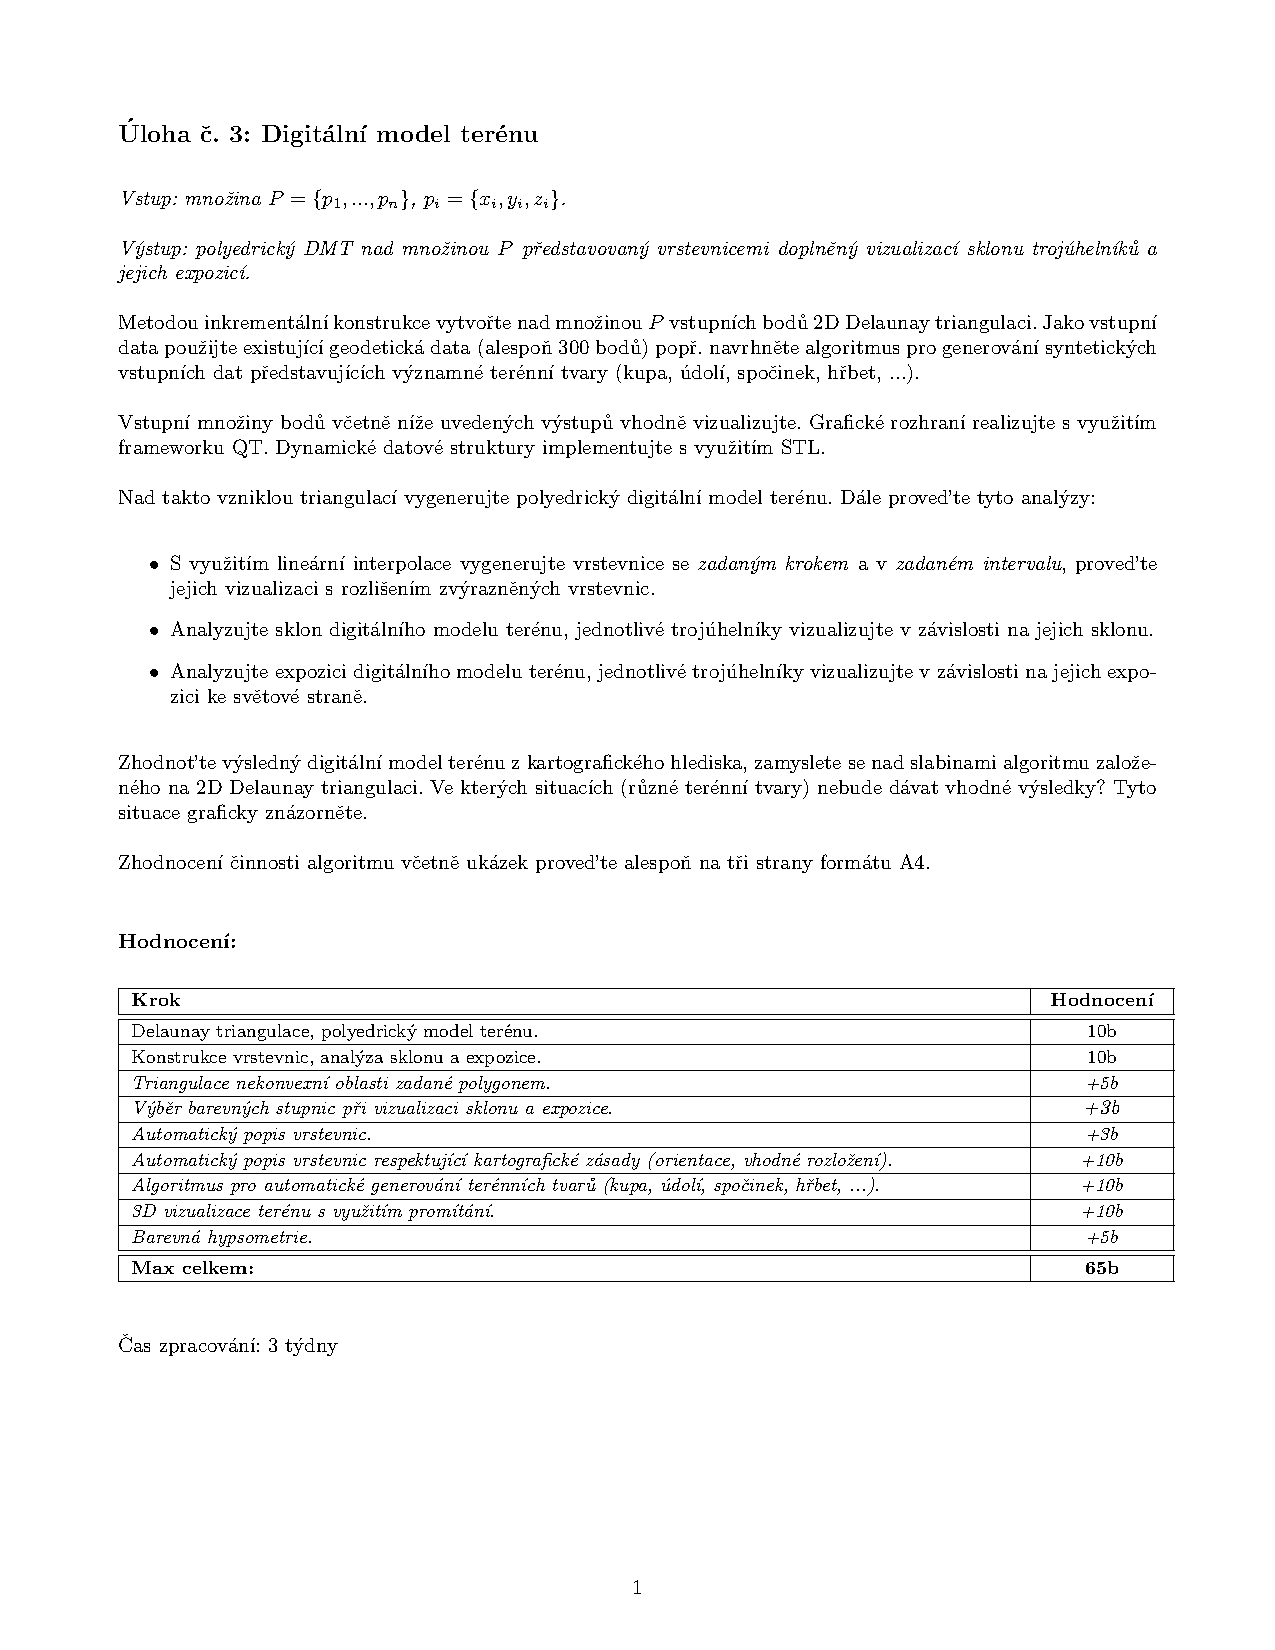
\includegraphics[clip, trim=0cm 4.5cm 0cm 3cm, width=1.0\textwidth]{./pictures/zadani03.pdf}
\end{figure}

V rámci této úlohy nebyly implementovány žádné bonusové úlohy.
\clearpage

\section{Popis a rozbor problému}
Úloha \textbf{Digitální model terénu a jeho analýzy} se zabývá vytvořením aplikace, která Delaunayho triangulací nad vstupní množinou bodů $P$ vytvoří trojúhelníkovou síť, pro kterou se lineární interpolací vypočítají vrstevnice. Aplikace dále počítá a vhodně vizualizuje sklon a expozici trojúhelníků ke světovým stranám.\\ 

Způsobů, jak geometricky zkonstruovat trojúhelníkovou síť, je více. Pro účely této úlohy byla vybrána Delaunayho triangulace, protože poskytuje optimální trojúhelníky z hlediska tvaru, což je zejména v kartografii velmi důležité. Delaunayho triangulace má čtyři základní vlastnosti:
\begin{enumerate}
\item Uvnitř kružnice opsané trojúhelníku $t_i \in DT$ neleží žádný jiný bod množiny $P$.
\item $DT$ maximalizuje minimální úhel v $\forall t_i$, avšak $DT$ neminimalizuje maximální úhel v $t_i$.
\item $DT$ je lokálně optimální i globálně optimální vůči kritériu minimálního úhlu.
\item $DT$ je jednoznačná, pokud žádné čtyři body neleží na kružnici.\footnote{Zdroj: \href{https://web.natur.cuni.cz/~bayertom/images/courses/Adk/adk5.pdf}{https://web.natur.cuni.cz}, slide 22}
\end{enumerate}

%\begin{figure}[h!]
	%\centering
	%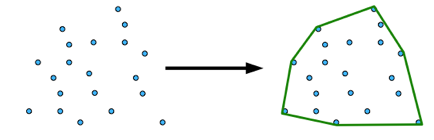
\includegraphics[width=13cm]{./pictures/ch.png}
	%\caption{Ukázka konvexní obálky (\href{http://mind.cs.byu.edu/courses/312/projects/project2_files/ConvexHull_python.php}{\textsl{zdroj}})}
%\end{figure}

\section{Algoritmy}
Tato kapitola se zabývá popisem algoritmů, které byly v aplikaci implementovány. 

\subsection{Delanuayho triangulace}
Delaunyho triangulace byla realizována inkrementální konstrukcí, která je založena na postupném přidávání bodů do již vytvořené triangulace. Během výpočtu je používaná struktura $AEL$ (Active Edge List), která obsahuje všechny hrany, proto které ještě nebyl nalezen třetí bod trojúhelníku. Hrana, pro kterou byl bod nalezen, je vzápětí ze seznamu odstraněna. Před přidáním hran do seznamu je kontrolováno, zda se v něm již nenachází hrana s opačnou orientací. V takovém případě není hrana do seznamu přidána.\\

Mějme množinu bodů $P$ a orientovanou hranu $e_i$. Hledáme takový bod $p_i \in P$, který se nachází v levé polorovině vymezené hranou $e_i$, pro který dále platí, že poloměr kružnice jemu a hraně opsané je minimální. Během výpočtu jsou upřednostňovány body, jejichž středy opsaných kružnic se nachází v pravé polorovině. Je-li bod splňující výše uvedené kritéria nalezen, vytvoří se dvě nové orientované hrany $e_{i+1}$ a $e_{i+2}$, které se přidají do triangulace a do $AEL$. Původní hrana $e_i$ je z $AEL$ odstraněna. Není-li žádný vhodný bod nalezen, dochází k prohození orientace hrany $e_i$ a postup je opakován. Celý proces je ukončen ve chvíli, kde se v $AEL$ nenachází již žádná hrana. \\ 

Zjednodušený zápis algoritmu lze zapsat způsobem uvedeným níže:

\begin{enumerate}
\item Nalezení pivota $a$: $a$ = min($x$) a jemu nejbližší bod $b$
\item Vytvoření $e_1 = (a,b)$
\item Nalezení Delaunayho bodu: $r(k_i)$ = min, $k_i = (e_1,p_i)$
\item Podmínka: $p_i$ nenalezen $\rightarrow e_1 = (b,a)$, opakuj krok 3
\item Vytvoř zbylé hrany trojúhelníku: $e_2 = (b,p_i)$, $e_3 = (p_i,a)$
\item Přidej hrany do $AEL$: $AEL \leftarrow e_1$, $AEL \leftarrow e_2$, $AEL \leftarrow e_3$
\item Přidej hrany do triangulace $DT$: $DT \leftarrow e_1$, $DT \leftarrow e_2$, $DT \leftarrow e_3$
\item Dokud $AEL \neq \emptyset$:
\subitem Vezmi první hranu z $AEL \rightarrow e_1$
\subitem Prohoď orientaci: $e_1 = (b,a)$
\subitem Nalezení Delaunayho bodu: $r(k_i)$ = min, $k_i = (e_1,p_i)$
\subitem Podmínka: $p_i$ nalezen 
\subsubitem Vytvoř zbylé hrany trojúhelníku: $e_2 = (b,p_i)$, $e_3 = (p_i,a)$
\subsubitem Přidej hranu do $DT$: $DT \leftarrow e_1$
\subsubitem $add(e_2,AEL,DT), add(e_3,AEL,DT)$
\end{enumerate}
~\\
Lokální algoritmus $add$:
\begin{enumerate}
\item Prohoď orientaci: $e' = (b,a)$
\item Podmínka: $e' \in AEL \rightarrow$ odstraň $e'$ z $AEL$
\item Jinak: $AEL \leftarrow e$  
\item $DT \leftarrow e$
\end{enumerate}

\subsection{Vrstevnice}
Druhý algoritmus použitý v aplikaci slouží k výpočtu vrstevnic. Vrstevnice byly zkonstruovány metodou lineární interpolace, která je založena na předpokladu, že spád terénu mezi dvěma body $p_i$ se mění stejně, tedy konstantně. Výpočet byl proveden postupně pro všechny trojúhelníky a vrstevnice byly ukládány jako seznam hran.\\

Mějme trojúhelník $t_i$ tvořený třemi hranami $e_{1}(p_{1},p_{2})$, $e_{2}(p_{2},p_{3})$ a $e_{3}(p_{3},p_{1})$ a rovinu $\rho$ o výšce Z. Hledáme průsečnici roviny trojúhelníku $t_i$ s rovinou $\rho$. Pro kritérium $t = (z-z_i)(z-z_{i+1})$ mohou nastat tři základní situace:

\begin{enumerate}
\item $t < 0 \rightarrow e_i \cap \rho$
\item $t > 0 \rightarrow e_i \notin \rho$ 
\item $t = 0 \rightarrow e_i \in \rho$
\end{enumerate}
~\\
Pro případy 2 a 3 nebyly vrstevnice řešeny. Nastane-li případ 1 ($e_i \cap \rho$), je pro hranu $e_i$ a rovinu $\rho$ níže uvedenými vzorci vypočten průsečík $a$ o výšce $z_a$: (pro přehlednost uvedeno pro hranu $e_1$)

$$ x_a = \frac{(x_2-x_1)}{(z_2-z_1)}(z-z_1)+x_1 $$
$$ y_a = \frac{(y_2-y_1)}{(z_2-z_1)}(z-z_1)+y_1 $$

\subsection{Sklon}
Algoritmus pro výpočet sklonu počítá sklon jednotlivých trojúhelníků $t_i$. Sklon je úhel $\varphi$ mezi svislicí $n$ a normálou trojúhelníku $n_t$. Rovina trojúhelníku $t_i$ je určena vektory $u$, $v$. Sklon nabývá hodnot $\textless$0$^\circ$;180$^\circ$???$\textgreater$ a v aplikaci je zobrazen v odstínech šedi.\\

$$n = (0,0,1)$$
$$n_t = \vec{u}\times \vec{v}$$
$$\varphi =\arccos(\frac{n_t \cdot n}{|n_t| |n|})$$

\subsection{Orientace}




\section{Problematické situace}
V algoritmu \textit{Sweep Line} bylo nutné ošetřit singularitu, která způsobovala generování nekonvexní obálky. Konkrétně bylo nutné odstranit duplicitní body. V opravené verzi aplikace je situace ošetřena setříděním bodů podle souřadnice X a porovnáním vzdáleností mezi dvěma po sobě jdoucími body. Je-li vzdálenosti menší než stanovená mez $\epsilon$, body jsou považovány za duplicitní a bod s větší souřadnicí X je ze vstupní množiny odstraněn. \\

Podmínka ($d_{p_i,p_j} < \epsilon$) $\rightarrow$ bod $p_j$ nezahrnut (viz. Obrázek 2)\\


Algoritmus \textit{Jarvis Scan} generuje špatné výsledky, není-li ošetřeno, že žádné tři body nejsou spolu kolineární. Tento problém se zejména projevoval při generaci setu \textit{Grid}, který jich obsahuje spoustu. Singularita byla ošetřena vypočtením úhlu $\sphericalangle p_{jj}, p_j, p_i$, a pokud byl menší, než stanovená mez $\epsilon$, byl pro další výpočty vybrán bližší z kolineárních bodů.

\begin{itemize}
\item Podmínka ($\sphericalangle p_{jj}, p_j, p_i$) $< \epsilon$
\subitem Podmínka ($d_{p_j,p_i} < d_{min}$) $\rightarrow$ vyber bod $p_i$, $d_{min} = d_{p_j,p_i}$
\end{itemize}

Dalším problémem bylo, jak zajistit, aby byl generovaný rastr pravidelný. To bylo ošetřeno zaokrouhlením počtu vstupních bodů směrem nahoru tak, aby po odmocnění vznikl pravidelný rastr.\\

počet bodů v řádce/sloupci = $roundUp(\sqrt{num\_of\_points})$

\section{Vstupní data}
Aplikace si na základě ručního zadání vstupních parametrů uživatelem sama vygeneruje potřebná vstupní data. Z rozbalovací nabídky \textbf{Shape of set} uživatel volí prostorové uspořádání generované množiny bodů. Na výběr jsou možnosti \textit{Random set}, \textit{Grid} a \textit{Circle}. V kolonce \textbf{Number of points} uživatel volí, kolik bodů bude generováno. Lze tak učinit buď přímým zadáním počtu bodů, nebo zvýšením/snížením počtu bodů o 1000 šipkami na boku. Aplikace omezuje minimální a maximální počet generovaných bodů na interval $\textless$1, 1000000$\textgreater$. Množina bodů se vygeneruje stisknutím tlačítka \textsl{Generate set}.\\

Uživatel má dále možnost volit, jaký výpočetní algoritmus bude použit pro tvorbu konvexní obálky. Rozbalovací nabídka \textbf{Method} nabízí celkem tři výpočetní algoritmy: \textit{Jarvis Scan}, \textit{Quick Hull} a \textit{Sweep Line}. Konvexní obálka je generována stisknutím tlačítka \textsl{Create CH}. Pokud před spuštěním procesu nebyla vygenerována žádná vstupní množina bodů, uživatel je upozorněn chybovou hláškou. 

\section{Výstupní data}
Vygenerovaná množina bodů a její konvexní obálka je vykreslena v grafickém okně aplikace. Aplikace dále vypisuje časy [ms], jak dlouho trvalo generování množiny a jak dlouho nad danou množinou běžel výpočetní algoritmus.\\

V rámci testování byly nad množinami bodů \textit{Random set}, \textit{Grid} a \textit{Circle} postupně spuštěny všechny tři algoritmy. Pro každou množinu a algoritmus byla pro daný počet bodů $n = \{1000, 5000, 10000, 25000, 50000, 75000, 100000, 200000, 500000, 1000000\}$ aplikace spuš\-tě\-na 10x, aby bylo získáno dostatečné množství testovacích dat. Z každé testované množiny bylo tedy získáno celkem 300 testovacích dat. Data byla ukládána do textového souboru a následně zpracována v \textit{Excelu}.


\clearpage
\section{Aplikace}
V následují kapitole je představen vizuální vzhled vytvořené aplikace tak, jak ji vidí prostý uživatel.

%\begin{figure}[h!]
	%\centering
	%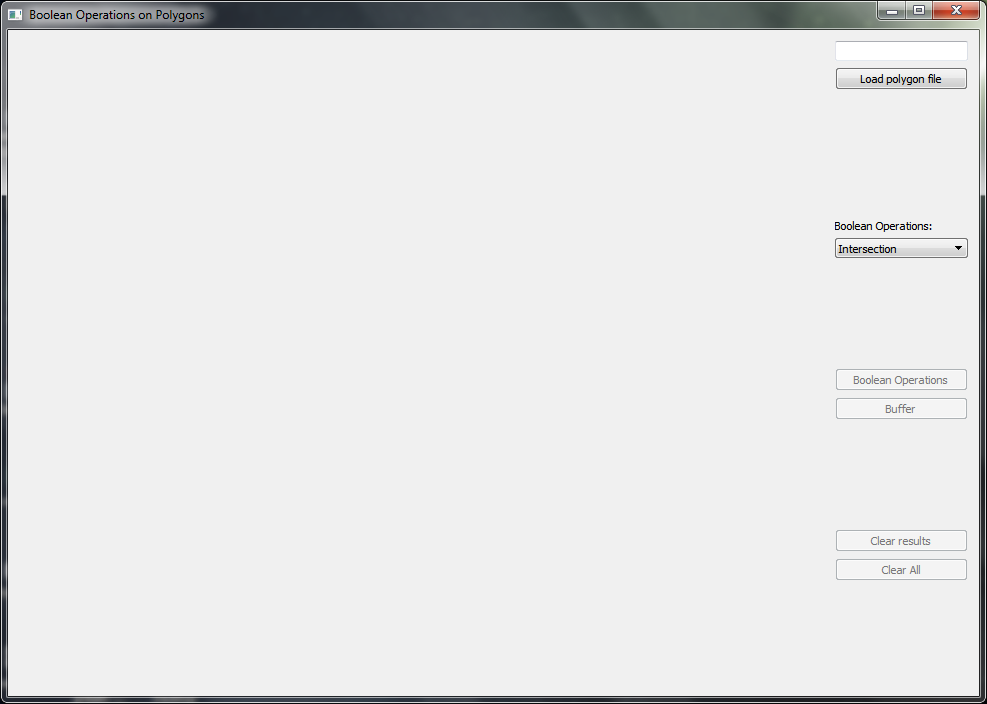
\includegraphics[width=11.5cm]{./pictures/app_default.png}
	%\caption{Výchozí vzhled aplikace po spuštění}
%\end{figure}



\clearpage
 
\section{Dokumentace}
Tato kapitola obsahuje dokumentaci k jednotlivým třídám.

\subsection{!Algorithms}
Třída \textit{Algorithms} obsahuje metody pro výpočet Delaunayho triangulace a analýzu DTM.

\subsubsection*{delaunayTriangulation}
Metoda \textbf{delaunayTriangulation} vytváří nad množinou bodů Delaunayho triangulaci. Na vstupu je vektor bodů typu \texttt{QPoint3D}, metoda vrací uspořádaný vektor hran \texttt{Edge}, které tvoří jednotlivé trojúhelníky.\\

\textbf{Input}:
\begin{itemize}
\item \textsl{vector} $\textless$\texttt{QPoint3D}$\textgreater$ $points$
\end{itemize}

\textbf{Output}:
\begin{itemize}
\item \textsl{vector} $\textless$\texttt{Edge}$\textgreater$
\end{itemize}

\subsubsection*{!createContours}
Metoda \textbf{createContours} vytváří nad vstupní množinou hran vrstevnice na základě zadané minimální a maximální výšky a kroku, po kterém se vrstevnice budou vykreslovat.  Metoda vrací vektor hran, které představují vrstevnice.\\

\textbf{Input}:
\begin{itemize}
\item \textsl{vector} $\textless$\texttt{Edge}$\textgreater$ $dt$
\item \texttt{double} $z\_min$ $\rightarrow$ minimální výška
\item \texttt{double} $z\_max$ $\rightarrow$ maximální výška
\item \texttt{double} $dz$ $\rightarrow$ krok vrstevnic
\end{itemize}

\textbf{Output}:
\begin{itemize}
\item \textsl{vector} $\textless$\texttt{Edge}$\textgreater$
\end{itemize}

\subsubsection*{!getSlope}
Metoda \textbf{getSlope} počítá sklon trojúhelníku, který je tvořen třemi body. Návratová hodnota typu \texttt{double} nabývá hodnot $\textless$0$^\circ$;180$^\circ$???$\textgreater$ a vrací sklon trojúhelníku.\\

\textbf{Input}:
\begin{itemize}
\item \texttt{QPoint3D} $p_1$
\item \texttt{QPoint3D} $p_2$
\item \texttt{QPoint3D} $p_3$
\end{itemize}

\subsubsection*{!getAspect}
Metoda \textbf{getSlope} počítá orientaci trojúhelníku, který je tvořen třemi body, ke světovým stranám. Návratová hodnota typu \texttt{double} vrací orientaci trojúhelníku ve stupních. Hodnota 0$^\circ$ je umístěna na xxx, orientace je pravotočiná/levotočivá.\\

\textbf{Input}:
\begin{itemize}
\item \texttt{QPoint3D} $p_1$
\item \texttt{QPoint3D} $p_2$
\item \texttt{QPoint3D} $p_3$
\end{itemize}

\subsubsection*{analyzeDTM}
Metoda \textbf{analyzeDTM} vytváří z vektoru hran trojúhelníky a počítá pro ně sklon a orientaci. Vypočtené hodnoty ukládá do datového typu \texttt{Triangle}. Návratová hodnota metody je vektor trojúhelníků typu \texttt{Triangle}.\\

\textbf{Input}:
\begin{itemize}
\item \textsl{vector} $\textless$\texttt{Edge}$\textgreater$ $dt$
\end{itemize}

\textbf{Output}:
\begin{itemize}
\item \textsl{vector} $\textless$\texttt{Triangle}$\textgreater$
\end{itemize}

\subsubsection*{getPointLinePosition}
Metoda \textbf{getPointLinePosition} určuje polohu bodu $q$ vzhledem k přímce tvořené dvěma body. Na vstupu jsou 3 body typu \texttt{QPoint3D}, návratová hodnota je nově definovaný typ \texttt{TPosition}.\\

\textbf{Input}:
\begin{itemize}
\item \texttt{QPoint3D} $q$
\item \texttt{QPoint3D} $a$
\item \texttt{QPoint3D} $b$
\end{itemize}

\textbf{Output}:
\begin{itemize}
\item \texttt{LEFT} $\rightarrow$ bod se nachází vlevo od přímky
\item \texttt{RIGHT} $\rightarrow$ bod se nachází vpravo od přímky
\item \texttt{ON} $\rightarrow$ bod se nachází na přímce
\end{itemize}

\subsubsection*{!getCircleRadius}
Metoda \textbf{getCircleRadius} počítá poloměr kružnice, která je tvořena 3 body. Na vstupu jsou 3 body typu \texttt{QPoint3D}, návratová hodnota typu \texttt{double} vrací velikost poloměru kružnice.\\ 

\textbf{Input}:
\begin{itemize}
\item \texttt{QPoint3D} $p_1$ 
\item \texttt{QPoint3D} $p_2$ 
\item \texttt{QPoint3D} $p_3$
\item !!!\texttt{QPoint3D} $c$
\end{itemize}

\subsubsection*{getDistance}
Metoda \textbf{getDistance} počítá vzdálenost mezi dvěma body. Na vstupu jsou 2 body typu \texttt{QPoint3D}, návratová hodnota typu \texttt{double} vrací vzdálenost mezi dvěma body.\\ 

\textbf{Input}:
\begin{itemize}
\item \texttt{QPoint3D} $p_1$ 
\item \texttt{QPoint3D} $p_2$
\end{itemize}

\subsubsection*{getNearestPoint}
Metoda \textbf{getNearestPoint} slouží k nalezení nejbližšího bodu z množiny bodů vzhledem k danému bodu $p$. Na vstupu je daný bod $p$ a vektor bodů typu \texttt{QPoint3D}. Návratová hodnota typu \texttt{int} vrací index nejbližšího bodu.

\textbf{Input}:
\begin{itemize}
\item \texttt{QPoint3D} $p$ 
\item \textsl{vector} $\textless$\texttt{QPoint3D}$\textgreater$ $points$
\end{itemize}

\subsubsection*{getDelaunayPoint}
Metoda \textbf{getDelaunayPoint} slouží k nalezení třetího bodu trojúhelníku, který splňuje Delaunayho kritérium nejmenší opsané kružnice. Na vstupu jsou dva body typu \texttt{QPoint3D}, které představují orientovanou hranu, a vektor bodů typu \texttt{QPoint3D}. Návratová hodnota typu \texttt{int} vrací index hledaného bodu.\\

\textbf{Input}:
\begin{itemize}
\item \texttt{QPoint3D} $s$ $\rightarrow$ počáteční bod hrany
\item \texttt{QPoint3D} $e$ $\rightarrow$ koncový bod hrany
\item \textsl{vector} $\textless$\texttt{QPoint3D}$\textgreater$ $points$
\end{itemize}

\subsubsection*{getContourPoint}
Metoda \textbf{getContourPoint} počítá průsečík hrany trojúhelníku tvořené dvěma body typu \texttt{QPoint3D} s rovinou o dané výšce Z. Návratová hodnota je typu \texttt{QPoint3D}.\\

\textbf{Input}:
\begin{itemize}
\item \texttt{QPoint3D} $p_1$ 
\item \texttt{QPoint3D} $p_2$ 
\item \texttt{double} $z$ 
\end{itemize}

\subsection{!Draw}
Třída \textit{Draw} obsahuje metody, které nahrávají a vykreslují vstupní množinu bodů. Dále zajišťuje vykreslení a smazání všech operací, kterou jsou nad množinou prováděny.

\subsubsection*{paintEvent}
Metoda \textbf{paintEvent} vykresluje vstupní množinu bodů, Delaunayho triangulaci, vrstevnice a sklon a orientaci trojúhelníků.

\subsubsection*{clearDT}
Metoda \textbf{clearDT} slouží k vymazání všech vykreslených dat.

\subsubsection*{getPoints}
Metoda \textbf{getPoints} slouží k získání vektoru bodů z kreslící plochy. Metoda vrací vektor bodů typu \texttt{QPoint3D}.

\subsubsection*{getDT}
Metoda \textbf{getPoints} slouží k získání vektoru hran z kreslící plochy. Metoda vrací vektor hran typu \texttt{Edge}.

\subsubsection*{setDT}
Metoda \textbf{setDT} slouží k převedení Delaunayho triangulace do kreslícího okna.

\subsubsection*{setContours}
Metoda \textbf{setContours} slouží k převedení vrstevnic do kreslícího okna.

\subsubsection*{setDTM}
Metoda \textbf{setDTM} slouží k převedení digitálního modelů terénu do kreslícího okna.

\subsubsection*{loadDTM}
Metoda \textbf{loadDTM} slouží k načtení vstupních dat do aplikace. Součástí metody je i kontrola, zda se soubor úspěšně nahrál. Návratová hodnota je typu \textsl{QString} vrací hlášku, zda byly polygony úspěšně nahrány čí nikoli.


\subsection{Edge}
Třída \textit{Edge} slouží k manipulaci s orientovanými hranami. Definuje dva body typu \texttt{QPoint3D} jako počáteční a koncový bod hrany.

\subsubsection*{getS}
Metoda \textbf{getS} slouží k získání počáteční body hrany. 

\subsubsection*{getE}
Metoda \textbf{getE} slouží k získání koncový body hrany. 

\subsubsection*{switchOrientation}
Metoda \textbf{switchOrientation} prohazuje orientaci hrany.  

\subsubsection*{????operator}


\subsection{QPpoint3D}
Třída \textbf{QPpoint3D} slouží k definování nového datového typu \texttt{QPoint3D}, který je odvozen od typu \texttt{QPointF} a který navíc obsahuje souřadnici Z.

\subsubsection*{getZ}
Metoda \textbf{getZ} slouží k získání souřadnice Z daného bodu.

\subsubsection*{setZ}
Metoda \textbf{setZ} slouží k nastavení souřadnice Z daného bodu. 


\subsection{SortByXAsc}
Třída \textbf{SortByXAsc} má na vstupu dva body typu \texttt{QPoint3D}, návratová hodnota je typu \texttt{bool}. Metoda vrací bod s nižší  souřadnicí X. Mají-li oba body shodnou souřadnici X, vrací bod s nižší souřadnicí Y.\\

\textbf{Input}:
\begin{itemize}
\item \texttt{QPoint3D} $p_1$
\item \texttt{QPoint3D} $p_2$
\end{itemize}

\textbf{Output}:
\begin{itemize}
\item 0 $\rightarrow$ bod $p_2$ má nižší $x$ souřadnici
\item 1 $\rightarrow$ bod $p_1$ má nižší $x$ souřadnici
\end{itemize}

\subsection{Triangle}
Třída \textbf{Triangle} slouží k definování nového datového typu \texttt{Triangle}, který v sobě uchovává informaci o třech bodech typu \texttt{QPoint3D}, které tvoří trojúhelník, a o sklonu a expozici trojúhelníku.

\subsubsection*{getPi}
Metoda \textbf{getSlope} slouží k získání bodu $P_i$ daného trojúhelníku. 

\subsubsection*{getSlope}
Metoda \textbf{getSlope} slouží k získání sklonu daného trojúhelníku. 

\subsubsection*{getAspect}
Metoda \textbf{getAspect} slouží k získání orientace daného trojúhelníku. 


\subsection{Widget}
Metody třídy \textbf{Widget} slouží pro práci uživatele s aplikací. Metody na vstupu nemají žádné parametry a návratové hodnoty jsou typu \texttt{void}.

\subsubsection*{on\_delaunay\_button\_clicked}
Metoda \textbf{on\_delaunay\_button\_clicked} nad vstupní množinou bodů zobrazí Delaunayho triangulaci. 

\subsubsection*{on\_clear\_button\_clicked}
Metoda \textbf{on\_clear\_button\_clicked} vrací aplikaci do výchozí polohy smazáním všeho, co bylo vykresleno. 

\subsubsection*{on\_contours\_button\_clicked}
Metoda \textbf{on\_contours\_button\_clicked} nad vygenerovanou trojúhelníkovou sítí z Delaunayho triangulace vykreslí vrstevnice. 

\subsubsection*{on\_dtm\_button\_clicked}
Metoda \textbf{on\_dtm\_button\_clicked} obarví trojúhelníky vygenerované Delaunayho triangulací v odstínech šedi podle hodnoty sklonu daného trojúhelníku.

\subsubsection*{!!!aspect}


\subsubsection*{on\_load\_button\_clicked}
Metoda \textbf{on\_load\_button\_clicked} načítá data z textového formátu. Uživatel sám vyhledává cestu k požadovanému souboru.


\clearpage
\section{Závěr}
V rámci úlohy \textit{Konvexní obálky} byla vytvořena aplikace, která nad vstupní množinou bodů vytváří striktně konvexní obálky. V rámci testování, která trvalo dlouho do noci a použitým počítačům dala pořádně zabrat, byla shromážděna data průměrné doby výpočtu striktně konvexní obálky pro jednotlivé algoritmy. Z časových důvodů byly implementovány jen některé bonusové úlohy. Opravená verze aplikace lépe implementuje odstraňo\-vá\-ní duplicitních bodů v algoritmu \textit{Sweep Line}, což výrazně přispělo ke snížení doby běhu algoritmu. V závislosti na tom byly upraveny hodnoty v tabulkách a grafy z nich vycházející.\\

Po nově provedeném opravném testování považujeme za nejvhodnější algoritmus pro výpočet konvexní obálky algoritmus \textit{Sweep Line}, a to i přesto, že pro množinu \textit{Grid} byl o něco málo rychlejší algoritmus \textit{Quick Hull}. Jeho rychlost se projevila hlavně u množiny \textit{Circle} (striktně konvexní obálku nad milionem bodů generoval průměrně pod desetinu sekundy). Pro množiny \textit{Random} a \textit{Grid} lze považovat algoritmus \textit{Quick Hull} za srovnatelný s algoritmem \textit{Sweep Line} co se týče výpočetní doby. Jeho slabina se však projevila u množiny \textit{Circle}, jejíž prostorové uspořádání zaručuje, že všechny body náleží konvexní obálce. Tady \textit{Quick Hull} trochu zaváhal a výpočtení doba se prodloužila. Jako nevyhovujícím pro tvorbu konvexních obálek byl shledán algoritmus \textit{Jarvis Scan}. Výpočet obálky mu i na malých množinách trval o poznání déle než ostatním algoritmům, avšak překvapila nás rychlost, s jakou se vypořádal s kružnicí v porovnání s jinými množinami.\\

Závěrem by bylo vhodné podotknout, že data z testování nejsou 100\% spolehlivá. Již v průběhu testování bylo zaznamenáno, že doba výpočtu algoritmu velmi závisí na výkonu použitého počítače (rozdíl v rychlostech byl až dvojnásobný) a také na tom, zda jsou v době testování na počítači spuštěny jiné aplikace (např. prohlížeč) nebo se provádí jiné úkony (např. psaní technické zprávy). To může být jednou z příčin vzniku odchylek a nepřesností, které se v datech občas vyskytují. Pro zachování přibližně konzistentních podmínek při testování byly použity dva notebooky s podobným výkonem.\\

Do budoucna by jistě šla rozšířit nabídka generovaných množin bodů a naprogramovat celková automatizace testování. Aktuální verze kódu pro testování obsahovala pouze cyklus na 10 opakování téhož výpočtu. Dále by mohl být naprogramován další výpočetní algoritmus, \textit{Graham Scan}, na který již autorky neměly čas. Mezi pozitivní přínosy úlohy zajisté patří objevení způsobu hromadného exportu grafů z \textit{Excelu} do formátu *.png.

\clearpage

\section{Zdroje}
\begin{enumerate}
\item  \textsl{BAYER, Tomáš. 2D triangulace, DMT} [online][cit. 4. 12. 2018].\\
Dostupné z: \href{https://web.natur.cuni.cz/~bayertom/images/courses/Adk/adk5.pdf}{https://web.natur.cuni.cz}

%\item  \textsl{CS 312 - Convex Hull Project} [online][cit. 10. 11. 2018].\\
%Dostupné z: \href{http://mind.cs.byu.edu/courses/312/projects/project2_files/ConvexHull_python.php}{http://mind.cs.byu.edu}


\end{enumerate}
\end{document}

%getCircleRadius c
%smazat datové typy z popisu a dát je jen do input/output
%hodnota sklonu
%getAspect orientace